        %%******************************************%%
        %%                                          %%
        %%        Modello di tesi di laurea         %%
        %%            di Andrea Giraldin            %%
        %%                                          %%
        %%             2 novembre 2012              %%
        %%                                          %%
        %%******************************************%%


% I seguenti commenti speciali impostano:
% 1. 
% 2. PDFLaTeX come motore di composizione;
% 3. tesi.tex come documento principale;
% 4. il controllo ortografico italiano per l'editor.

% !TEX encoding = UTF-8
% !TEX TS-program = pdflatex
% !TEX root = tesi.tex
% !TEX spellcheck = it-IT

\documentclass[10pt,                    % corpo del font principale
               a4paper,                 % carta A4
               twoside,                 % impagina per fronte-retro
               openright,               % inizio capitoli a destra
               english,                 
               italian,                 
               ]{book}    

%**************************************************************
% Importazione package
%************************************************************** 

%\usepackage{amsmath,amssymb,amsthm}    % matematica

\usepackage[T1]{fontenc}
\usepackage{lmodern}               % codifica dei font:
                                        % NOTA BENE! richiede una distribuzione *completa* di LaTeX

\usepackage[utf8]{inputenc}             % codifica di input; anche [latin1] va bene
                                        % NOTA BENE! va accordata con le preferenze dell'editor

\usepackage[english, italian]{babel}    % per scrivere in italiano e in inglese;
                                        % l'ultima lingua (l'italiano) risulta predefinita

\usepackage{bookmark}                   % segnalibri

\usepackage{caption}                    % didascalie

\usepackage{chngpage,calc}              % centra il frontespizio

\usepackage{csquotes}                   % gestisce automaticamente i caratteri (")

\usepackage{emptypage}                  % pagine vuote senza testatina e piede di pagina

\usepackage{epigraph}			% per epigrafi

\usepackage{eurosym}                    % simbolo dell'euro

%\usepackage{indentfirst}               % rientra il primo paragrafo di ogni sezione

\usepackage{graphicx}                   % immagini

\usepackage{hyperref}                   % collegamenti ipertestuali

\usepackage[binding=5mm]{layaureo}      % margini ottimizzati per l'A4; rilegatura di 5 mm

\usepackage{listings}                   % codici

\usepackage{microtype}                  % microtipografia

\usepackage{mparhack,relsize}  % finezze tipografiche

\usepackage{nameref}                    % visualizza nome dei riferimenti                                      

\usepackage[font=small]{quoting}        % citazioni

\usepackage{subfig}                     % sottofigure, sottotabelle

\usepackage[italian]{varioref}          % riferimenti completi della pagina

\usepackage[dvipsnames]{xcolor}         % colori

\usepackage{booktabs}                   % tabelle                                       
\usepackage{tabularx}                   % tabelle di larghezza prefissata                                    
\usepackage{longtable}                  % tabelle su più pagine                                        
\usepackage{ltxtable}                   % tabelle su più pagine e adattabili in larghezza

\usepackage[toc, acronym]{glossaries}   % glossario
                                        % per includerlo nel documento bisogna:
                                        % 1. compilare una prima volta tesi.tex;
                                        % 2. eseguire: makeindex -s tesi.ist -t tesi.glg -o tesi.gls tesi.glo
                                        % 3. eseguire: makeindex -s tesi.ist -t tesi.alg -o tesi.acr tesi.acn
                                        % 4. compilare due volte tesi.tex.

\usepackage[backend=biber,style=verbose-ibid,hyperref,backref]{biblatex}
                                        % eccellente pacchetto per la bibliografia; 
                                        % produce uno stile di citazione autore-anno; 
                                        % lo stile "numeric-comp" produce riferimenti numerici
                                        % per includerlo nel documento bisogna:
                                        % 1. compilare una prima volta tesi.tex;
                                        % 2. eseguire: biber tesi
                                        % 3. compilare ancora tesi.tex.

%**************************************************************
% file contenente le impostazioni della tesi
%**************************************************************

%**************************************************************
% Frontespizio
%**************************************************************

% Autore
\newcommand{\myName}{Riccardo Montagnin}                                    
\newcommand{\myTitle}{Titolo della tesi}

% Tipo di tesi                   
\newcommand{\myDegree}{Tesi di laurea triennale}

% Università             
\newcommand{\myUni}{Università degli Studi di Padova}

% Facoltà       
\newcommand{\myFaculty}{Corso di Laurea in Informatica}

% Dipartimento
\newcommand{\myDepartment}{Dipartimento di Matematica "Tullio Levi-Civita"}

% Titolo del relatore
\newcommand{\profTitle}{Prof.}

% Relatore
\newcommand{\myProf}{Tullio Vardanega}

% Luogo
\newcommand{\myLocation}{Padova}

% Anno accademico
\newcommand{\myAA}{2016-2017}

% Data discussione
\newcommand{\myTime}{Luglio 2017}


%**************************************************************
% Impostazioni di impaginazione
% see: http://wwwcdf.pd.infn.it/AppuntiLinux/a2547.htm
%**************************************************************

\setlength{\parindent}{14pt}   % larghezza rientro della prima riga
\setlength{\parskip}{0pt}   % distanza tra i paragrafi


%**************************************************************
% Impostazioni di biblatex
%**************************************************************
\bibliography{bibliografia} % database di biblatex 

\defbibheading{bibliography} {
    \cleardoublepage
    \phantomsection 
    \addcontentsline{toc}{chapter}{\bibname}
    \chapter*{\bibname\markboth{\bibname}{\bibname}}
}

\setlength\bibitemsep{1.5\itemsep} % spazio tra entry

\DeclareBibliographyCategory{opere}
\DeclareBibliographyCategory{web}

\addtocategory{opere}{womak:lean-thinking}
\addtocategory{web}{site:agile-manifesto}

\defbibheading{opere}{\section*{Riferimenti bibliografici}}
\defbibheading{web}{\section*{Siti Web consultati}}


%**************************************************************
% Impostazioni di caption
%**************************************************************
\captionsetup{
    tableposition=top,
    figureposition=bottom,
    font=small,
    format=hang,
    labelfont=bf
}

%**************************************************************
% Impostazioni di glossaries
%**************************************************************

\usepackage{glossaries}
\makeglossaries
%INIZIO NOME
%\newglossaryentry{nome}{
%	name={nome},
%	description={descrizione}
%}
%FINE NOME

%INIZIO UML
\newglossaryentry{UML}{
	name={UML},
	description={\\ Unified Modeling Language, linguaggio di modellizzazione e specifica basato sul paradigma orientato agli oggetti}
}
\newglossaryentry{API}{
	name={API},
	description={\\ Acronimo di Application Programming Interface (ovvero interfaccia di programmazione
		di una applicazione) si indicano un unsieme di procedure (raggruppate assieme per
		formare un insieme di strumenti specifici) per il compimento di un determinato compito
		all’interno di un certo programma}
}
\newglossaryentry{iframe}{
	name={iframe},
	description={L'iframe in informatica è un elemento HTML. Si tratta infatti di un frame "ancorato" all'interno della pagina, equivale cioè ad un normale frame, ma con la differenza di essere un elemento inline (interno) della pagina, non esterno.
	L'iframe viene generalmente utilizzato per mostrare il contenuto di una pagina web, o di una qualsivoglia risorsa, all'interno di un riquadro in una seconda pagina principale}
}
\newglossaryentry{SPA}{
	name={SPA},
	description={Single Page Application è una metologià per la creazione delle interfacce web. In questo caso esiste una sola pagina HTML, tutto il resto(navigazione, pagine) viene gestito  tramite Javascript. I più famosi framework/librerie sono Angular, React e Vue }
}
\newglossaryentry{framework}{
	name={framework},
	description={Un framework è un'architettura logica di supporto (spesso un'implementazione logica di un particolare design pattern) su cui un software può essere progettato e realizzato, spesso facilitandone lo sviluppo da parte del programmatore. Inoltre fornisce una raccolta di librerie ed oggetti già fatti}
}
\newglossaryentry{MVC}{
	name={MVC},
	description={Model-view-controller in informatica, è un pattern architetturale molto diffuso nello sviluppo di sistemi software, in particolare nell'ambito della programmazione orientata agli oggetti, in grado di separare la logica di presentazione dei dati dalla logica di business}
}
\newglossaryentry{MVVM}{
	name={MVVM},
	description={
	Una variante del pattern MVC è MVVM, Model View ViewModel. Questo pattern propone un ruolo più attivo della View rispetto a MVC: la View è in grado di gestire eventi, eseguire operazioni ed effettuare il data-binding. In questo contesto, quindi, alcune delle funzionalità del Controller vengono inglobate nella View, la quale si appoggia su un’estensione del Model: il ViewModel.
	Il ViewModel è quindi un Model esteso con funzionalità per la manipolazione dei dati e per l’interazione con la View}
}
\newglossaryentry{design pattern}{
	name={design pattern},
	description={Questo termine fa riferimento a una soluzione progettuale generale ad un problema
		ricorrente che può presentarsi in diverse situazioni durante le fasi di progettazione e
		sviluppo del software}
}
\newglossaryentry{W3C Recommendation}{
	name={W3C Recommendation},
	description={La parola W3C significa World Wide Web Consortium, cioè il Consorzio Internazionale che si occupa di definire linee guida e standard non proprietari, le tecnologie, i protocolli e tutto quanto necessario per lo sviluppo del Web }
}
\newglossaryentry{Javascript}{
	name={Javascript},
	description={JavaScript è un linguaggio di scripting orientato agli oggetti e agli eventi, comunemente utilizzato nella programmazione Web lato client per la creazione, in siti web e applicazioni web, di effetti dinamici interattivi tramite funzioni di script invocate da eventi innescati a loro volta in vari modi dall'utente sulla pagina web in uso}
}
\newglossaryentry{EMCAScript 6}{
	name={EMCAScript 6},
	description={Spesso conoscitto con acronimo ES6 è una versione del linguaggio di scripting Javascript standardizzata }
}
\newglossaryentry{UI}{
	name={UI},
	description={User Interface è un'interfaccia uomo-macchina, ovvero ciò che si frappone tra una macchina e un utente, consentendone l'interazione reciproca}
}
\newglossaryentry{serverless}{
	name={serverless},
	description={Nel contesto dell'applicazone, serverless è un metodo di creazione ed esecuzione di applicazioni e servizi che non richiede la gestione dell'infrastruttura. L'applicazione sarà comunque eseguita su server, ma la gestione di quest'ultimo sarà a carico di AWS }
}



\newglossaryentry{mock}{
	name={mock},
	description={Dal inglese "finto". Utilizzato nello sviluppo per simulare il comportamento degli oggetti reali, in questo modo è possibile provare delle parti di un sistema senza necessariamente implementare tutto}
}

\newglossaryentry{repository}{
	name={repository},
	description={E' un ambiente condiviso di sviluppo software. In generale è una cartella condivisa da molti utenti nel quale è posibile lavorare insieme in maniera molto semplice}
}
\newglossaryentry{SDK}{
	name={SDK},
	description={Acronimo di Software Development Kit, si riferisce genericamente a un insieme di
		strumenti per migliorare lo sviluppo o la documentazione di software}
}



\newglossaryentry{JSON}{
	name={JSON},
	description={Acronimo di JavaScript Object Notation, è un formato dichiarativo basato sullo
	Standard ECMA-262 adatto all’interscambio di dati fra applicazioni client-server}
}


\newglossaryentry{Observer}{
	name={Observer},
	description={E' un design patter che sta alla base di MVC, permette a molti oservatori di oservare un unica fonte di verità. In questo modo tutti gli oggetti hanno i stessi dati}
}


\newglossaryentry{Decorator}{
	name={Decorator},
	description={Decorator è un design pattern che permette di decorare un'oggetto utilizzando le funzioni d'altri oggetti. Utilizzato per diminuire l'esagerato utilizzato dell' ereditarietà. }
}

\newglossaryentry{Singleton}{
	name={Singleton},
	description={Singleton è un design pattern che permette di creare un unica isatanza di un'oggetto in tutta l'applicazione}
}

\newglossaryentry{DI}{
	name={DI},
	description={Acronimo di Dependency Injection, è un design pattern che risolve il problema di dipendenze. Utilizzato soprattutto nella programmazione ad oggetti, dove spesso molti oggetti contengono altri oggetti come parametri. Questo pattern permette di iniettare le dipendeze tra gli oggetti invece di avere le istanze interne, in questo modo ogni oggetto può essere modificato senza causare danni in altri oggetti}
} % database di termini
\makeglossaries


%**************************************************************
% Impostazioni di graphicx
%**************************************************************
\graphicspath{{immagini/}} % cartella dove sono riposte le immagini


%**************************************************************
% Impostazioni di hyperref
%**************************************************************
\hypersetup{
    %hyperfootnotes=false,
    %pdfpagelabels,
    %draft,	% = elimina tutti i link (utile per stampe in bianco e nero)
    colorlinks=true,
    linktocpage=true,
    pdfstartpage=1,
    pdfstartview=FitV,
    % decommenta la riga seguente per avere link in nero (per esempio per la stampa in bianco e nero)
    %colorlinks=false, linktocpage=false, pdfborder={0 0 0}, pdfstartpage=1, pdfstartview=FitV,
    breaklinks=true,
    pdfpagemode=UseNone,
    pageanchor=true,
    pdfpagemode=UseOutlines,
    plainpages=false,
    bookmarksnumbered,
    bookmarksopen=true,
    bookmarksopenlevel=1,
    hypertexnames=true,
    pdfhighlight=/O,
    %nesting=true,
    %frenchlinks,
    urlcolor=webbrown,
    linkcolor=RoyalBlue,
    citecolor=webgreen,
    %pagecolor=RoyalBlue,
    %urlcolor=Black, linkcolor=Black, citecolor=Black, %pagecolor=Black,
    pdftitle={\myTitle},
    pdfauthor={\textcopyright\ \myName, \myUni, \myFaculty},
    pdfsubject={},
    pdfkeywords={},
    pdfcreator={pdfLaTeX},
    pdfproducer={LaTeX}
}

%**************************************************************
% Impostazioni di itemize
%**************************************************************
\renewcommand{\labelitemi}{$\ast$}

%\renewcommand{\labelitemi}{$\bullet$}
%\renewcommand{\labelitemii}{$\cdot$}
%\renewcommand{\labelitemiii}{$\diamond$}
%\renewcommand{\labelitemiv}{$\ast$}


%**************************************************************
% Impostazioni di listings
%**************************************************************
\lstset{
    language=[LaTeX]Tex,%C++,
    keywordstyle=\color{RoyalBlue}, %\bfseries,
    basicstyle=\small\ttfamily,
    %identifierstyle=\color{NavyBlue},
    commentstyle=\color{Green}\ttfamily,
    stringstyle=\rmfamily,
    numbers=none, %left,%
    numberstyle=\scriptsize, %\tiny
    stepnumber=5,
    numbersep=8pt,
    showstringspaces=false,
    breaklines=true,
    frameround=ftff,
    frame=single
} 


%**************************************************************
% Impostazioni di xcolor
%**************************************************************
\definecolor{webgreen}{rgb}{0,.5,0}
\definecolor{webbrown}{rgb}{.6,0,0}


%**************************************************************
% Altro
%**************************************************************

\newcommand{\omissis}{[\dots\negthinspace]} % produce [...]

% eccezioni all'algoritmo di sillabazione
\hyphenation
{
    ma-cro-istru-zio-ne
    gi-ral-din
}

\newcommand{\sectionname}{sezione}
\addto\captionsitalian{\renewcommand{\figurename}{Figura}
                       \renewcommand{\tablename}{Tabella}}

\newcommand{\glsfirstoccur}{\ap{{[g]}}}

\newcommand{\intro}[1]{\emph{\textsf{#1}}}

%**************************************************************
% Environment per ``rischi''
%**************************************************************
\newcounter{riskcounter}                % define a counter
\setcounter{riskcounter}{0}             % set the counter to some initial value

%%%% Parameters
% #1: Title
\newenvironment{risk}[1]{
    \refstepcounter{riskcounter}        % increment counter
    \par \noindent                      % start new paragraph
    \textbf{\arabic{riskcounter}. #1}   % display the title before the 
                                        % content of the environment is displayed 
}{
    \par\medskip
}

\newcommand{\riskname}{Rischio}

\newcommand{\riskdescription}[1]{\textbf{\\Descrizione:} #1.}

\newcommand{\risksolution}[1]{\textbf{\\Soluzione:} #1.}

%**************************************************************
% Environment per ``use case''
%**************************************************************
\newcounter{usecasecounter}             % define a counter
\setcounter{usecasecounter}{0}          % set the counter to some initial value

%%%% Parameters
% #1: ID
% #2: Nome
\newenvironment{usecase}[2]{
    \renewcommand{\theusecasecounter}{\usecasename #1}  % this is where the display of 
                                                        % the counter is overwritten/modified
    \refstepcounter{usecasecounter}             % increment counter
    \vspace{10pt}
    \par \noindent                              % start new paragraph
    {\large \textbf{\usecasename #1: #2}}       % display the title before the 
                                                % content of the environment is displayed 
    \medskip
}{
    \medskip
}

\newcommand{\usecasename}{UC}

\newcommand{\usecaseactors}[1]{\textbf{\\Attori Principali:} #1. \vspace{4pt}}
\newcommand{\usecasepre}[1]{\textbf{\\Precondizioni:} #1. \vspace{4pt}}
\newcommand{\usecasedesc}[1]{\textbf{\\Descrizione:} #1. \vspace{4pt}}
\newcommand{\usecasepost}[1]{\textbf{\\Postcondizioni:} #1. \vspace{4pt}}
\newcommand{\usecasealt}[1]{\textbf{\\Scenario Alternativo:} #1. \vspace{4pt}}

%**************************************************************
% Environment per ``namespace description''
%**************************************************************

\newenvironment{namespacedesc}{
    \vspace{10pt}
    \par \noindent                              % start new paragraph
    \begin{description} 
}{
    \end{description}
    \medskip
}

\newcommand{\classdesc}[2]{\item[\textbf{#1:}] #2}                     % file con le impostazioni personali

\begin{document}
%**************************************************************
% Materiale iniziale
%**************************************************************
\frontmatter
% !TEX encoding = UTF-8
% !TEX TS-program = pdflatex
% !TEX root = ../tesi.tex

%**************************************************************
% Frontespizio 
%**************************************************************
\begin{titlepage}

\begin{center}

\begin{LARGE}
\textbf{\myUni}\\
\end{LARGE}

\vspace{10pt}

\begin{Large}
\textsc{\myDepartment}\\
\end{Large}

\vspace{10pt}

\begin{large}
\textsc{\myFaculty}\\
\end{large}

\vspace{30pt}
\begin{figure}[htbp]
\begin{center}

\includegraphics[height=6cm]{logo-unipd}
\end{center}
\end{figure}
\vspace{30pt} 

\begin{LARGE}
\begin{center}
\textbf{\myTitle}\\
\end{center}
\end{LARGE}

\vspace{10pt} 

\begin{large}
\textsl{\myDegree}\\
\end{large}

\vspace{40pt} 

\begin{large}
\begin{flushleft}
\textit{Relatore}\\ 
\vspace{5pt} 
\profTitle \myProf
\end{flushleft}

\vspace{0pt} 

\begin{flushright}
\textit{Laureando}\\ 
\vspace{5pt} 
\myName
\end{flushright}
\end{large}

\vspace{40pt}

\line(1, 0){338} \\
\begin{normalsize}
\textsc{Anno Accademico \myAA}
\end{normalsize}

\end{center}
\end{titlepage} 
% !TEX encoding = UTF-8
% !TEX TS-program = pdflatex
% !TEX root = ../tesi.tex

%**************************************************************
% Colophon
%**************************************************************
\clearpage
\phantomsection
\thispagestyle{empty}

\hfill

\vfill

\noindent\myName: \textit{\myTitle,}
\myDegree,
\textcopyright\ \myTime.
% !TEX encoding = UTF-8
% !TEX TS-program = pdflatex
% !TEX root = ../tesi.tex

%**************************************************************
% Sommario
%**************************************************************
\cleardoublepage
\phantomsection
\pdfbookmark{Sommario}{Sommario}
\begingroup
\let\clearpage\relax
\let\cleardoublepage\relax
\let\cleardoublepage\relax

\chapter*{Sommario}
Il presente documento descrive il lavoro svolto durante il periodo di stage(dal 03/06/2018 al 03/08/2018), della durata di circa 320 ore, dal laureando Singh Parwinder presso l'azienda Nextep alla sede di Cittadella.
\\
In questo documento verranno descritte in dettaglio come è stata fatta  l'analisi dei requisiti, la progettazione, l'implementazione e la validazione dell'applicazione CS-template. L'applicazione in questione è stata realizzata utilizzando le tecnologie web innovative sia per quanto riguarda il lato frontend dell'applicazione che quello backend.\\
L'intero lavoro è stato svolto in ambiente Linux Ubuntu 18.04 LTS. Tutti i diagrammi delle classi e dei package sono conformi allo standard UML 2.0. Per realizzarli è stato usato il software Astah
Professional\footcite{http://astah.net/editions/professional}.  

%\vfill
%
%\selectlanguage{english}
%\pdfbookmark{Abstract}{Abstract}
%\chapter*{Abstract}
%
%\selectlanguage{italian}


\begin{description}
	\item[{\hyperref[cap:introduzione]{Il primo capitolo}}] descrive l’azienda ospitante.
	
	\item[{\hyperref[cap:progetto]{Il secondo capitolo}}] descrive il progetto d stage e le motivazioni della scelta.
	
	\item[{\hyperref[cap:Tecnologie utilizzate]{Il terzo capitolo}}] descrive le tecnologie utilizzate durante
	tutto il periodo di stage.

	\item[{\hyperref[cap:progettazione]{Il quarto capitolo}}] illustra ad l'intero periodo di stage. Dalla analisi dei requisiti fino alla validazione finale. 	
	
	\item[{\hyperref[cap:conclusioni]{Il quinto capitolo}}] conclusione e risultati ottenuti.
	
	\item[{\hyperref[cap:conclusioni]{Nel ultimo capitolo}}] viene riportato il glossario ed alcuni concetti secondo me molto interessanti.
\end{description}
Riguardo la stesura del testo, relativamente al documento sono state adottate le seguenti convenzioni tipografiche:
\begin{itemize}
	\item gli acronimi, le abbreviazioni e i termini ambigui o di uso non comune menzionati vengono definiti nel glossario, situato alla fine del presente documento;
	\item per la prima occorrenza dei termini riportati nel glossario viene utilizzata la seguente nomenclatura: \gls{API};
	\item i termini in lingua straniera o facenti parti del gergo tecnico sono evidenziati con il carattere \emph{corsivo}.
\end{itemize}
\endgroup			
%\glsfirstoccur
\vfill


% !TEX encoding = UTF-8
% !TEX TS-program = pdflatex
% !TEX root = ../tesi.tex

%**************************************************************
% Ringraziamenti
%**************************************************************
\cleardoublepage
\phantomsection
\pdfbookmark{Ringraziamenti}{ringraziamenti}
\begingroup
\let\clearpage\relax
\let\cleardoublepage\relax
\let\cleardoublepage\relax

\chapter*{Ringraziamenti}

\noindent \textit{Innanzitutto, vorrei esprimere la mia gratitudine al Prof. Francesco Ranzato, relatore della mia tesi, per l'aiuto e il sostegno fornitomi durante la stesura del lavoro.}\\

\noindent \textit{Desidero ringraziare con affetto i miei genitori per il sostegno, il grande aiuto e per essermi stati vicini in ogni momento durante gli anni di studio.}\\

\noindent \textit{Ho desiderio di ringraziare poi i miei amici per tutti i bellissimi anni passati insieme e le mille avventure vissute.}\\
\bigskip

\noindent\textit{\myLocation, \myTime}
\hfill \myName

\endgroup


% !TEX encoding = UTF-8
% !TEX TS-program = pdflatex
% !TEX root = ../tesi.tex

%**************************************************************
% Indici
%**************************************************************
\cleardoublepage
\pdfbookmark{\contentsname}{tableofcontents}
\setcounter{tocdepth}{2}
\tableofcontents
%\markboth{\contentsname}{\contentsname} 
\clearpage

\begingroup 
    \let\clearpage\relax
    \let\cleardoublepage\relax
    \let\cleardoublepage\relax
    %*******************************************************
    % Elenco delle figure
    %*******************************************************    
    \phantomsection
    \pdfbookmark{\listfigurename}{lof}
    \listoffigures

    \vspace*{8ex}

    %*******************************************************
    % Elenco delle tabelle
    %*******************************************************
    \phantomsection
    \pdfbookmark{\listtablename}{lot}
    \listoftables
        
    \vspace*{8ex}
\endgroup

\cleardoublepage

\cleardoublepage

%**************************************************************
% Materiale principale
%**************************************************************
\mainmatter
% !TEX encoding = UTF-8
% !TEX TS-program = pdflatex
% !TEX root = ../tesi.tex

%**************************************************************
\chapter{Introduzione}
\label{cap:introduzione}
In questo capitolo viene brevemente descritta l’azienda ospitante in cui è stata
svolta l’attività di stage e una descrizione ad alto livello del progetto realizzato.

%\emph{api}
%\noindent Esempio di utilizzo di un termine nel glossario \\


%\noindent Esempio di citazione in linea \\
%\cite{site:agile-manifesto}. \\

%\noindent Esempio di citazione nel pie' di pagina \\
%\footcite{http://www.zero12.it/} \\

%**************************************************************
\section{Dominio aziendale}
\subsection{L'azienda ospitante}
Nextep è una società fondata nel 2000 da Marco De Toni e Mirco Soffia, con sede
attuale a Cittadella (PD).
Opera nel settore informatico e si occupa di servizi web, web marketing e di infrastrutture
per gestire le informazioni delle aziende, e più in generale ha come obiettivo
quello di migliorare l’efficacia delle strategie di comunicazione web, delle aziende,
dedicando particolare attenzione alla reputazione e all’identità digitale. \\ \\
Nextep fa parte del gruppo Allos, insieme ad Allos Italia\footcite{https://www.allos.it/}, Allos Sud Africa\footcite{http://www.allos.co.za/}, Allos
USA\footcite{http://www.allosamerica.com/} e Zero12\footcite{http://www.zero12.it/}.
Allos si occupa di progetti e tecnologie per lo sviluppo del capitale umano, mentre
Zero12 si occupa dello sviluppo di soluzioni mobile e cloud based.
Il gruppo Allos è stato recentemente acquisito da EOH Holdings Ltd\footcite{http://www.eoh.co.za/}, una grande
società sudafricana.\\ \\
Nextep ha un organico di circa venti persone, tra dipendenti e collaboratori, con
varie competenze: grafici, sviluppatori, esperti di web marketing e tecnici. Sono presenti
tre gruppi principali di lavoro: quello di sviluppo, creativo e del supporto
tecnico.
In Nextep c’è un ambiente di lavoro giovane, dinamico ma allo stesso tempo professionale,
ed è incentivata la collaborazione e la condivisione di conoscenze e idee
tra le persone. Tutto questo favorisce sia la crescita individuale, dal punto di vista
professionale, che la crescita e l’amalgamazione dei vari gruppi di lavoro.
\begin{figure}[!h] 
	\centering 
	
\includegraphics[width=0.7\columnwidth]{azienda} 
	\caption{Logo di Nextep: immagine tratta dal sito dell’azienda}
\end{figure}
%**************************************************************
\subsection{Prodotti e servizi}
Nextep lavora per clienti di diversa tipologia e conformazione, dalla piccola impresa
privata alla multinazionale che si sta espandendo ulteriormente, e con questo offre
svariati prodotti e servizi in base alle esigenze e alle opportunità del mercato e proprie. 
\\ \\La maggior parte dei progetti riguarda la realizzazione di portali e siti web, ma vengono
sviluppati anche diversi altri prodotti, tra cui soluzioni e-commerce e applicazioni
mobile, sviluppo di progetti di virtualizzazione, e storage networking. Inoltre negli ultimi mesi l'azienda si sta dedicato molto anche ai prodotti di \emph{machine learning}, come i chatbot. \\ \\Nextep offre diversi tipi di servizi tra questi l'installazione e assistenza del portale di \emph{customer service} Zendesk. Guida le diverse società(piccole o grandi) verso la gestione dei proprio cliente in maniera semplice ed efficace. 
%**************************************************************

\section{Lo stage}
Il progetto di stage è consistito principalmente nella realizzazione di una applicazione per la piattaforma di \emph{customer service} Zendesk. La piattaforma Zendesk permette a un'aziedna di gestire tutte le richieste(chiamate \emph{tickets}) di propri clienti in unico posto. \\ L'applicazione realizzata permette agli agenti(persone che gestiscono le richieste dei clienti) e agli amministratori di Zendesk di realizzare contenuti(chiamati template) HTML e CSS in maniera molto semplice e veloce, ovvero utilizzando un editor \emph{drag-and-drop}. I template successivamente sono utilizzati nelle risposte verso i clienti. Questo permette di risparmiare una notevole quantità di tempo e non è necessario avere le conoscenze di HTML e CSS. Diverse aziende(clienti di Nextep) hanno fatta la richiesta esplicitamente di tale applicazione. .
\\
\\
Dopo una breve analisi insieme al tutor aziendale è stata definita la seguente struttura dell'applicazione ad alto livello: 
\begin{itemize}
	\item L'applicazione deve essere realizzata utilizzando Angular; 
	\item Oltre all'applicazione che dovrà essere integrata su Zendesk, è richiesta la realizzazione(sempre in Angular) anche di una pagina di \emph{admin} per la gestione di tutti i clienti che utilizzeranno tale applicazione;
	\item La pagina di \emph{admin} deve essere accessibile solo dopo aver effettuato il \emph{login};
	\item Il backend dell'applicazione deve essere tutto realizzato nei sistemi Cloud(AWS, Azure ecc.).
\end{itemize} 
             % Introduzione
% !TEX encoding = UTF-8
% !TEX TS-program = pdflatex
% !TEX root = ../tesi.tex

%**************************************************************
\chapter{Il progetto di stage}
In questo capitolo viene presentato il progetto di stage e le motivazioni della scelta.
\section{La piattaforma Zendesk}
\begin{figure}[!h] 
	\centering 
	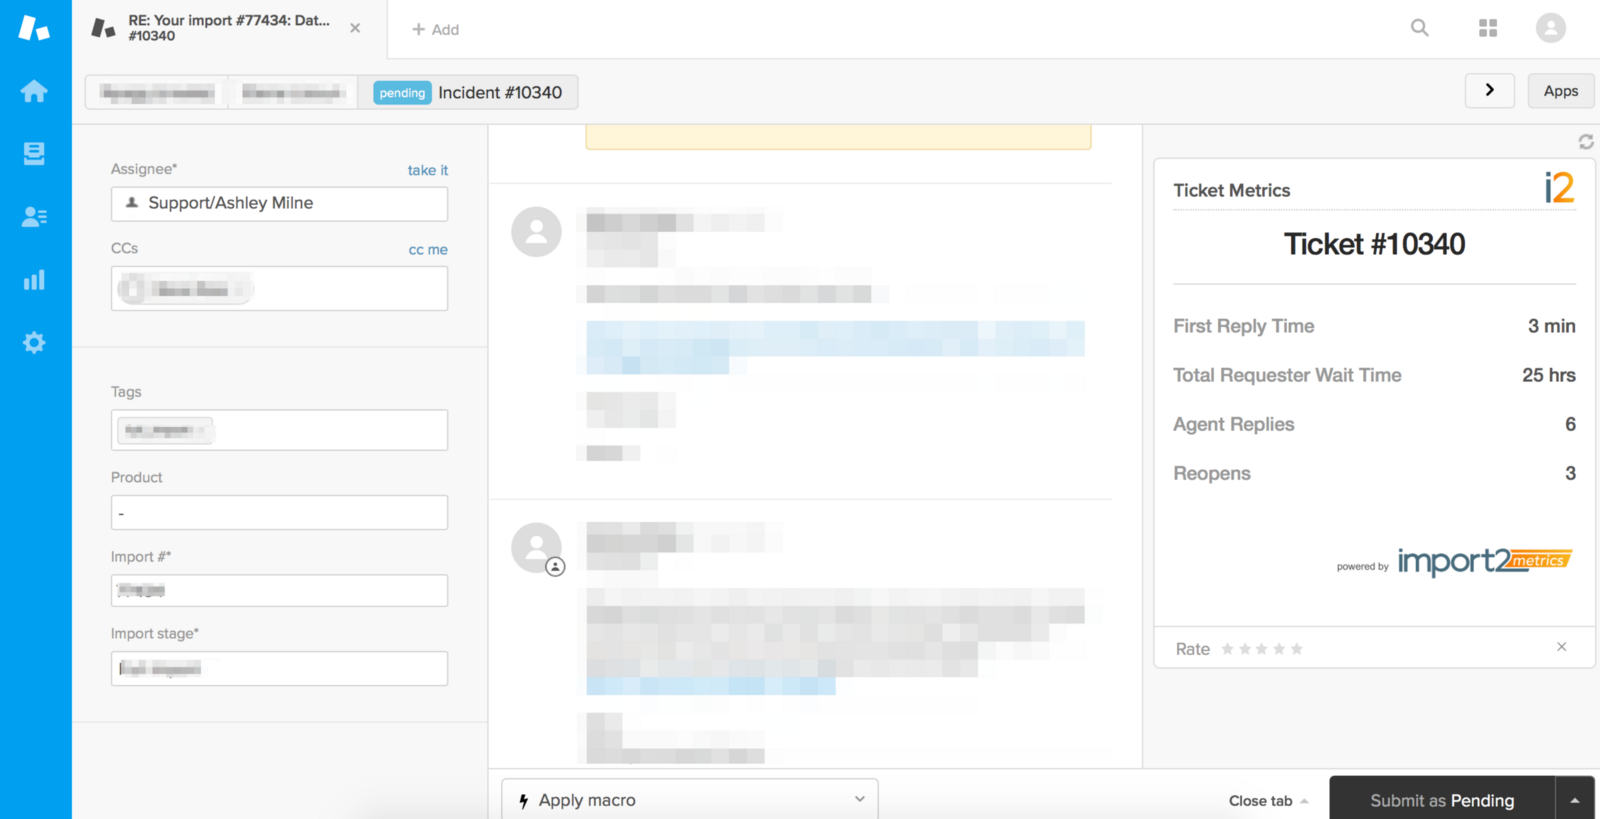
\includegraphics[width=0.8\columnwidth]{zendesk} 
	\caption{L'interfaccia utente Zendesk}
\end{figure}
Zendesk è una piattaforma online che permette a un'azienda di gestire le richieste provenienti da qualsiasi parte (mail, twitter, chat, ecc) dei proprio clienti in un unico posto sottoforma di tickets. E' la piattafroam più utilizzata al mondo dalle aziende per quanto rigurada l'assitenza online. Il posto forte di questa piattaforma sta proprio nella sua semplicità. Presenta un'interfaccia molto userfrendly, dopo un paio di ore una persona prende completa confidenza con i strumenti da essa offerti. Gli utenti sono divisi in 2 cattegorie:
	\begin{itemize}
		\item Gli agenti: un agente si occupa di elaborare le richieste dei clienti. 
		\item Gli amministratori: un amministraore di Zendesk si occupa di gestire gli agenti e tutta la piattaforna. 
	\end{itemize}
\newpage
Zendesk inoltre offre ottimi strumenti per realizzare applicazioni esterne oppure integrarle nella piattaforma come app. Uno sviluppatore può realizzare una app di Zendesk utilizzando qualsiasi tecnologia web. L'applicazione realizzata può essere utilizzata sulla propria piattaforma come una app privata, oppure caricata nel marketplace di Zendesk a pagamento o gratuitamente.  
 
\begin{figure}[!h] 
	\centering 
	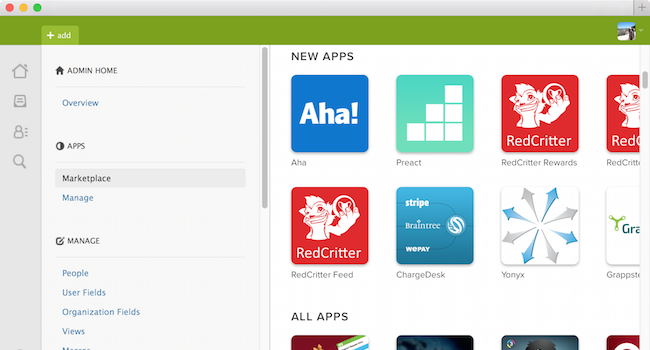
\includegraphics[width=0.8\columnwidth]{market} 
	\caption{Zendesk marketplace}
	\end{figure}

Il customer service via internet è un ambito sempre più in crescità, ci sono sempre più attività che si stanno spostando in internet. Un'attività di media dimenzione riceve al giorno in medai dai 500 a sopra le 1000 richieste dei clienti al giorno. La gestione con strumenti sbaglaiti di queste richieste può portare l'azienda a una notevole spesa(persona/lavoro) e soprattutto un feedback negativo dai clienti. 
\section{Lo stage}
Il progetto di stage è consistito principalmente nella realizzazione di una applicazione per la piattaforma di \emph{customer service} Zendesk. \\ L'applicazione realizzata permette agli agenti(persone che gestiscono le richieste dei clienti) e agli amministratori di Zendesk di realizzare contenuti(chiamati template) HTML e CSS in maniera molto semplice e veloce, ovvero utilizzando un editor \emph{drag-and-drop}. I template successivamente sono utilizzati nelle risposte verso i clienti. Questo permette di risparmiare una notevole quantità di tempo e non è necessario avere le conoscenze di HTML e CSS. Diverse aziende(clienti di Nextep) hanno fatta la richiesta esplicitamente di tale applicazione.
\\
\\
Alcuni dei benifici dell'applicazione CS-template:
\begin{itemize}
	\item realizzazione dei contenuti HTML e CSS senza sapere questi due linguaggi;
	\item la velocità con qui è possibile realizzare questi contenuti;
	\item permette agli agenti di realizzare le email predefinite, per rispondere alle richieste ricorrenti con un semplice click.
\end{itemize}
\newpage
\section{ Obiettivi dello stage}
Dopo una breve analisi insieme al tutor aziendale è sono stati definiti  seguenti obbietivi da raggiungere: 
\begin{itemize}
	\item apprendimento delle tecnologie necessarie per lo svolgimento del progetto;
	\item l'applicazione per la piattaforma Zendesk deve essere realizzata utilizzando Angular; 
	\item deve essere realizzata(sempre in Angular) anche una pagina degli \emph{admin} per la gestione di tutti i clienti che utilizzeranno tale applicazione;
	\item la pagina degli \emph{admin} deve essere accessibile solo dopo aver effettuato il \emph{login};
	\item il backend dell'applicazione deve essere tutto realizzato nei sistemi Cloud(AWS, Azure ecc.);
	\item tutta la progettazione deve essere documentata.
\end{itemize} 

\section{Interesse personale nello stage}

Avendo partecipato all’evento StageIT, organizzato dal corso di laurea in collaborazione
con confindustria Padova, ho potuto incontrare molte aziende, e ho quindi avuto a
disposizione molte proposte di stage da valutare.
\\

Ho cercato allora di sfruttare quest’occasione al meglio, ricercando tra le proposte
quella che mi sembrasse sia più interessante, sia che mi desse la possibilità di fare
esperienza ed imparare. Ero molto interessato ai framework/librerie moderni per la realizzazioni delle applicazioni web. Quindi ho cercato di puntare di più alle aziende che offrivano un'oppurtunità di stage con queste tipo di tecnologie. 
\\

Di seguito sono elencate le altre aziende e i  progetti di mio interesse dopo stage-it:
\begin{itemize}
	\item \textbf{Datasoil:} è una startup a Piombino Dese che si occupa di IoT(Internet of things). Il progetto proposto mi dava la possibilità di realizzare un applicazione web con React. Il problema principale di questo progetto era lo stack tecnologico molto limitato. Avrei realizzato solo la parte frontend dell'applicazione;
	\item \textbf{Thron:} è una azienda a Piazzola sul brenta. Il progetto consisteva nella realizzazione di una applicazione mobile utilizzando Vuejs(un framework simile ad Angular). Anche in questo caso, avrei lavorato solo nel lato frontend dell'applicazione. 
\end{itemize}
Ho scelto Nextep e il progetto CS-template soprattuto per lo stack tecnologico. In questo modo ho avuto la possibilità di studiare tecnologie sia lato frontend che lato backend di mie interesse. 
             % Processi
% !TEX encoding = UTF-8
% !TEX TS-program = pdflatex
% !TEX root = ../tesi.tex

%**************************************************************
\chapter{Descrizione dello stage}
\label{cap:descrizione-stage}
%**************************************************************

\intro{Breve introduzione al capitolo}\\

%**************************************************************
\section{Introduzione al progetto}

%**************************************************************
\section{Analisi preventiva dei rischi}

Durante la fase di analisi iniziale sono stati individuati alcuni possibili rischi a cui si potrà andare incontro.
Si è quindi proceduto a elaborare delle possibili soluzioni per far fronte a tali rischi.\\

\begin{risk}{Performance del simulatore hardware}
    \riskdescription{le performance del simulatore hardware e la comunicazione con questo potrebbero risultare lenti o non abbastanza buoni da causare il fallimento dei test}
    \risksolution{coinvolgimento del responsabile a capo del progetto relativo il simulatore hardware}
    \label{risk:hardware-simulator} 
\end{risk}

%**************************************************************
\section{Requisiti e obiettivi}


%**************************************************************
\section{Pianificazione}             % Kick-Off
% !TEX encoding = UTF-8
% !TEX TS-program = pdflatex
% !TEX root = ../tesi.tex

%**************************************************************
\chapter{Analisi dei requisiti}
\label{cap:analisi-requisiti}
Il presente capitolo ha come scopo quello di fornire una descrizione completa e precisa di tutti i requisitiG individuati e dei casi d’uso ad alto livello riguardanti il progetto CS-Template.

\section{Casi d'uso}

Per lo studio dei casi di utilizzo del prodotto sono stati creati dei diagrammi.
I diagrammi dei casi d'uso (in inglese \emph{Use Case Diagram}) sono diagrammi di tipo \gls{uml} dedicati alla descrizione delle funzioni o servizi offerti da un sistema, così come sono percepiti e utilizzati dagli attori che interagiscono col sistema stesso.
Ogni caso d’uso è definito secondo la seguente struttura:
\begin{itemize}
	\item Nome: Il titolo del caso d’uso;
	\item Attori: Indica gli attori principali e secondari del caso d’uso. In tutto il contesto
	dell’applicazione gli autori del sistema saranno così classificati:
	\begin{itemize}
		\item Utente Zendesk: sono gli utenti della piattaforma Zendesk. Possono essere gli agenti(persone che gestiscono le richieste dei cleinti) oppure gli amministratore di Zendesk;
		\item Utente generico: utente qualsiasi che non ha ancora effettuato l'accesso alla pagina degli amministratori;
		 \item Amministratore: utente amministratore Nextep, che ha compito di gestire tutti le aziende che utilizzano l'applicazione CS-Template.
	\end{itemize}

	\item Descrizione: Riporta una breve descrizione del caso d’uso;
	\item Precondizione: Specifica le condizioni che sono identificate come vere prima
	del verificarsi degli eventi del caso d’uso;
	\item Postcondizione: Specifica le condizioni che sono identificate come vere dopo il
	verificarsi degli eventi del caso d’uso.

\end{itemize}

\subsection{ Casi d'uso pagina degli amministratori}
Questa è la pagina web il cui scopo principale è quello di visualizzare la lista di tutti i clienti di Nextep che hanno l'applicazione CS-Template installata sulla propria piattaforma Zendesk. Inoltre permette di aggiungerne dei nuovi. L'accesso a questa pagina è garantita solo agli uenti amministratori di Nextep con le credenziali valide.
\begin{usecase}{1}{Login pagina amministratori}

	\usecaseactors{Utente generico}
	\usecasedesc{Caso d'uso descrive login alla pagina degli amministratori. }
	\usecasepre{L'utente non autenticato}
	\usecasepost{Il sistema riconosce l'utente amministratore}
		\begin{figure}[!h] 
		\centering 
		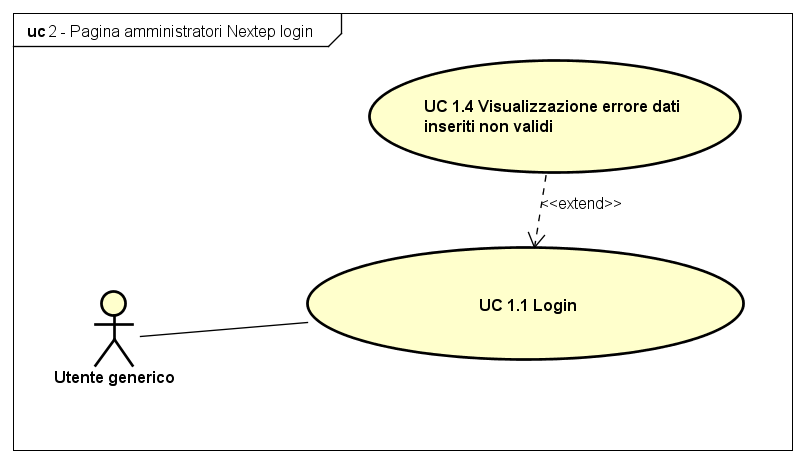
\includegraphics[width=1\columnwidth]{usecase/login} 
		\caption{UC 1 - pagina login}
	\end{figure}
\\ 
\\
\begin{usecase}{2}{Pagina degli amministratori}
	
	\usecaseactors{Nextep Admin}
	\usecasedesc{Caso d'uno descrive le funzionalità della pagina degli amministratori di Nextep. In questa pagina è possibile gestire tutti i clienti(aziende) di Nextep che utilizzano l'applicazione CS-Template}
	\usecasepre{Il sistema riconosce l'amministratore}
	\usecasepost{L’amministratore visualizza una lista di tutti i clienti(utilizzatori di CS-Template) registrati  nel  sistema,  visualizzando  per  ognuno  di  essi tutte le   informazioni  e un form per aggiungerne uno nuovo}
	\begin{figure}[!h] 
		\centering 
		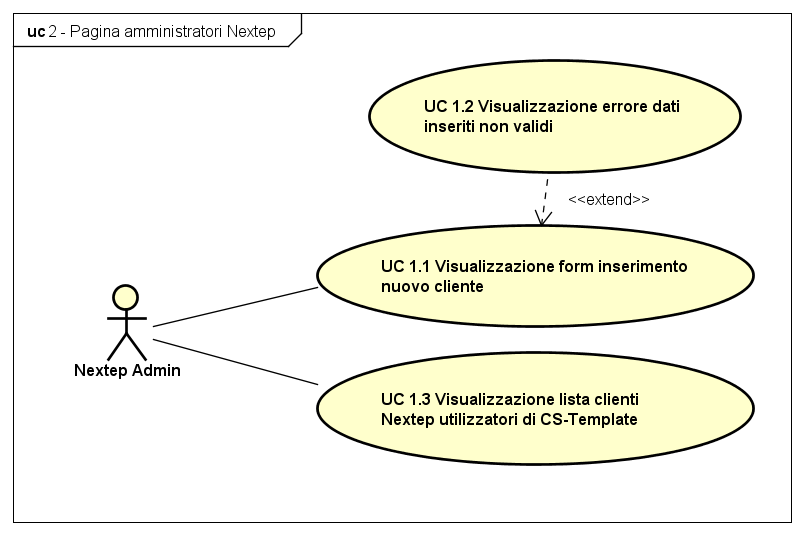
\includegraphics[width=1\columnwidth]{usecase/paginaAdmin} 
		\caption{UC 2 - funzionalità pagina admin}
	\end{figure}
\end{usecase}
\newpage
\subsection{ Casi d'uso pagina contenente l'editor drag-and-drop}
Questa pagina web contiene l'editor drag-and-drop che verrà visualizzato successivamente nella piattaforma Zendesk in un iframe. In seguito è riportato un caso d'uso generico che descrive tutte le proprietà ad alto livello dell'editor.
\begin{usecase}{3}{Editor drag-and-drop}
	
	\usecaseactors{Utente Zendesk}
	\usecasedesc{Caso d'uso descrive tutte le funzionalità ad alto livello che l'editor dovrà fornire}
	\usecasepre{L'utente Zendesk apre l'editor}
	\usecasepost{L'editor permette all'utente Zendesk di realizzare qualsiasi tipo di contentuto HTML e CSS}
	\begin{figure}[!h] 
		\centering 
		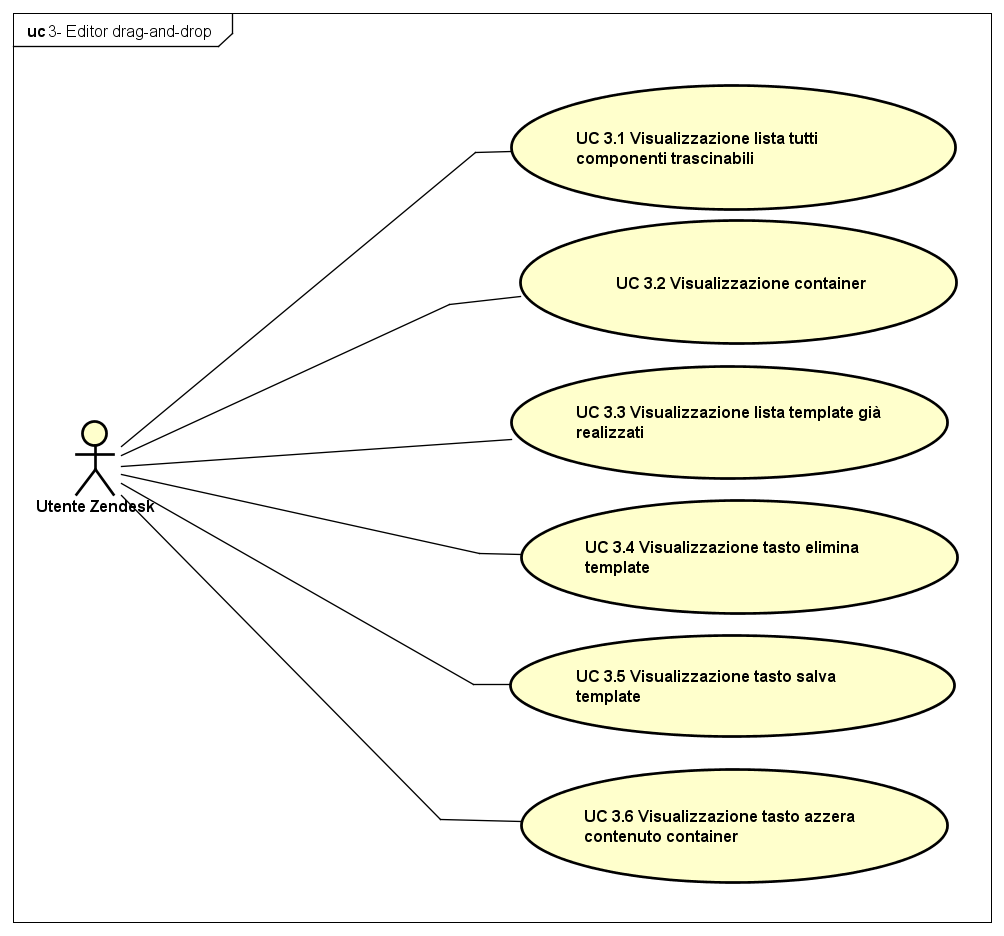
\includegraphics[width=1\columnwidth]{usecase/editor} 
		\caption{UC3 - pagina contenene l'editor}
	\end{figure}
\end{usecase}
\newpage
\subsection{ Casi d'uso pagina contenente il widget}
Questa pagina web contiene il widget che verrà visualizzato successivamente nella piattaforma Zendesk in un iframe. Il widget verrà mostrato quando verrà aperto una richeista qualsiasi del cliente. Esso permette di scegliere da una lista il contenuto HTML e CSS da utilizzare come risposta verso il cliente. 
\begin{usecase}{4}{Widget dei template}
	
	\usecaseactors{Utente Zendesk}
	\usecasedesc{Caso d'uso descrive tutte le funzionalità ad alto livello che il widget dovrà fornire}
	\usecasepre{L'utente Zendesk apre il widget}
	\usecasepost{Utente Zendesk sceglie il template da inviare come risposta al cliente}
	\begin{figure}[!h] 
		\centering 
		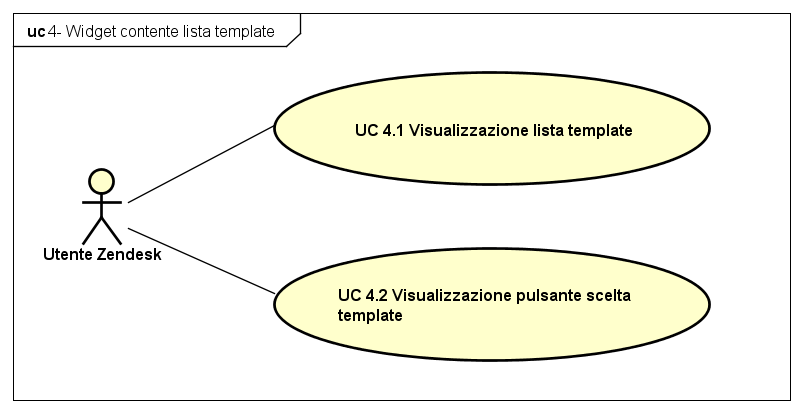
\includegraphics[width=1.2\columnwidth]{usecase/widget} 
		\caption{UC3 - pagina contenente il widget}
	\end{figure}
\\
\\
\\
\\
\\
\end{usecase}

\section{Tracciamento dei requisiti}

Da un'attenta analisi dei requisiti e degli use case effettuata sul progetto è stata stilata la tabella che traccia i requisiti in rapporto agli use case.\\
Sono stati individuati diversi tipi di requisiti e si è quindi fatto utilizzo di un codice identificativo per distinguerli.\\
Il codice dei requisiti è così strutturato R(F/Q/V)(N/D/O) dove:
\begin{enumerate}
	\item[R =] requisito
    \item[F =] funzionale
    \item[N =] obbligatorio (necessario)
    \item[D =] desiderabile
    \item[Z =] opzionale
\end{enumerate}

Nelle tabelle \ref{tab:requisiti-funzionali} e \ref{tab:requisiti-vincolo} sono riassunti i requisiti e il loro tracciamento con gli use case delineati in fase di analisi.
\\
\begin{table}%
\caption{Tabella del tracciamento dei requisti funzionali}
\label{tab:requisiti-funzionali}
\begin{tabularx}{\textwidth}{lXl}
\hline\hline
\textbf{Requisito} & \textbf{Descrizione} & \textbf{Use Case}\\
\hline
RFN-1   & Personale di Nextep può effetuare il login nella pagina degli amministraori & UC1 \\
\hline
RFN-2   & Nextep Admin può ottenere una lista con tutte le informazioni dei clienti che utilizzano l'applicazione CS-Template & UC2 \\
\hline
RFN-3   & Nextep Admin può eliminare un cliente dalla lista & UC2 \\
\hline
RFN-4   & Nextep Admin può aggiungere un nuovo cliente nella lista & UC2 \\
\hline
RFN-4   & Utente Zendesk può utilizzare l'editor drag-and-drop & UC3 \\
\hline
RFN-5   & Utente Zendesk può creare nuovi template & UC3 \\
\hline
RFN-6   & Utente Zendesk può salvare il template creato & UC3 \\
\hline
RFN-7   & Utente Zendesk può eliminare template creati & UC3 \\
\hline
RFN-8   & Utente Zendesk può azzerrare il contenuto del editor & UC3 \\
\hline
RFN-10   & Utente Zendesk può impostare il nome del template & UC3 \\
\hline
RFN-11   & Utente Zendesk può utilizzare il temaplte creato nella risposta verso il cliente & UC4 \\
\hline
RFD-12   & Utente Zendesk può esportare tutto i template creati in un file json come backup & UC4 \\
\hline
RFD-13   & Utente Zendesk può importare i template da un file json precedentemente creato & UC4 \\
\hline
\end{tabularx}
\end{table}%

\begin{table}%
\caption{Tabella del tracciamento dei requisiti di vincolo}
\label{tab:requisiti-vincolo}
\begin{tabularx}{\textwidth}{lXl}
\hline\hline
\textbf{Requisito} & \textbf{Descrizione} & \textbf{Use Case}\\
\hline
RVO-1    & Il backend dell'applicazioend deve essere realizzato utilizzando gli servizi cloud & - \\
\hline
RVO-2    & L'applicazione deve essere utilizzabile solo dai clienti aggiunti da Nextep, implementando un sistema d' accesso tramite il token & - \\
\hline
RVO-3    & L’intero progetto deve essere accompagnato da
documentazione completa & - \\
\hline
\end{tabularx}
\end{table}%             % Concept Preview
% !TEX encoding = UTF-8
% !TEX TS-program = pdflatex
% !TEX root = ../tesi.tex

%**************************************************************
\chapter{Progettazione}
\label{cap:progettazione}
\label{sec:tecnologie-strumenti}

In questo capitolo vengono illustrate le strategie di progettazione adottate per la realizzazione del prodotto in questione. La progettazione viene descritta ad alto livello senza descrivere in dettaglio tutti i diagrammi delle classi. 

\section{Progettazione Frontend}
\label{sec:progettazione}

\subsection{Atomic design}
Creata da Brad Frost nel 2013, l'Atomic design è una metodologia composta da 5 differenti fasi, utile per creare un sistema di interfacce in maniera gerarchica.
\begin{figure}[!h] 
	\centering 
	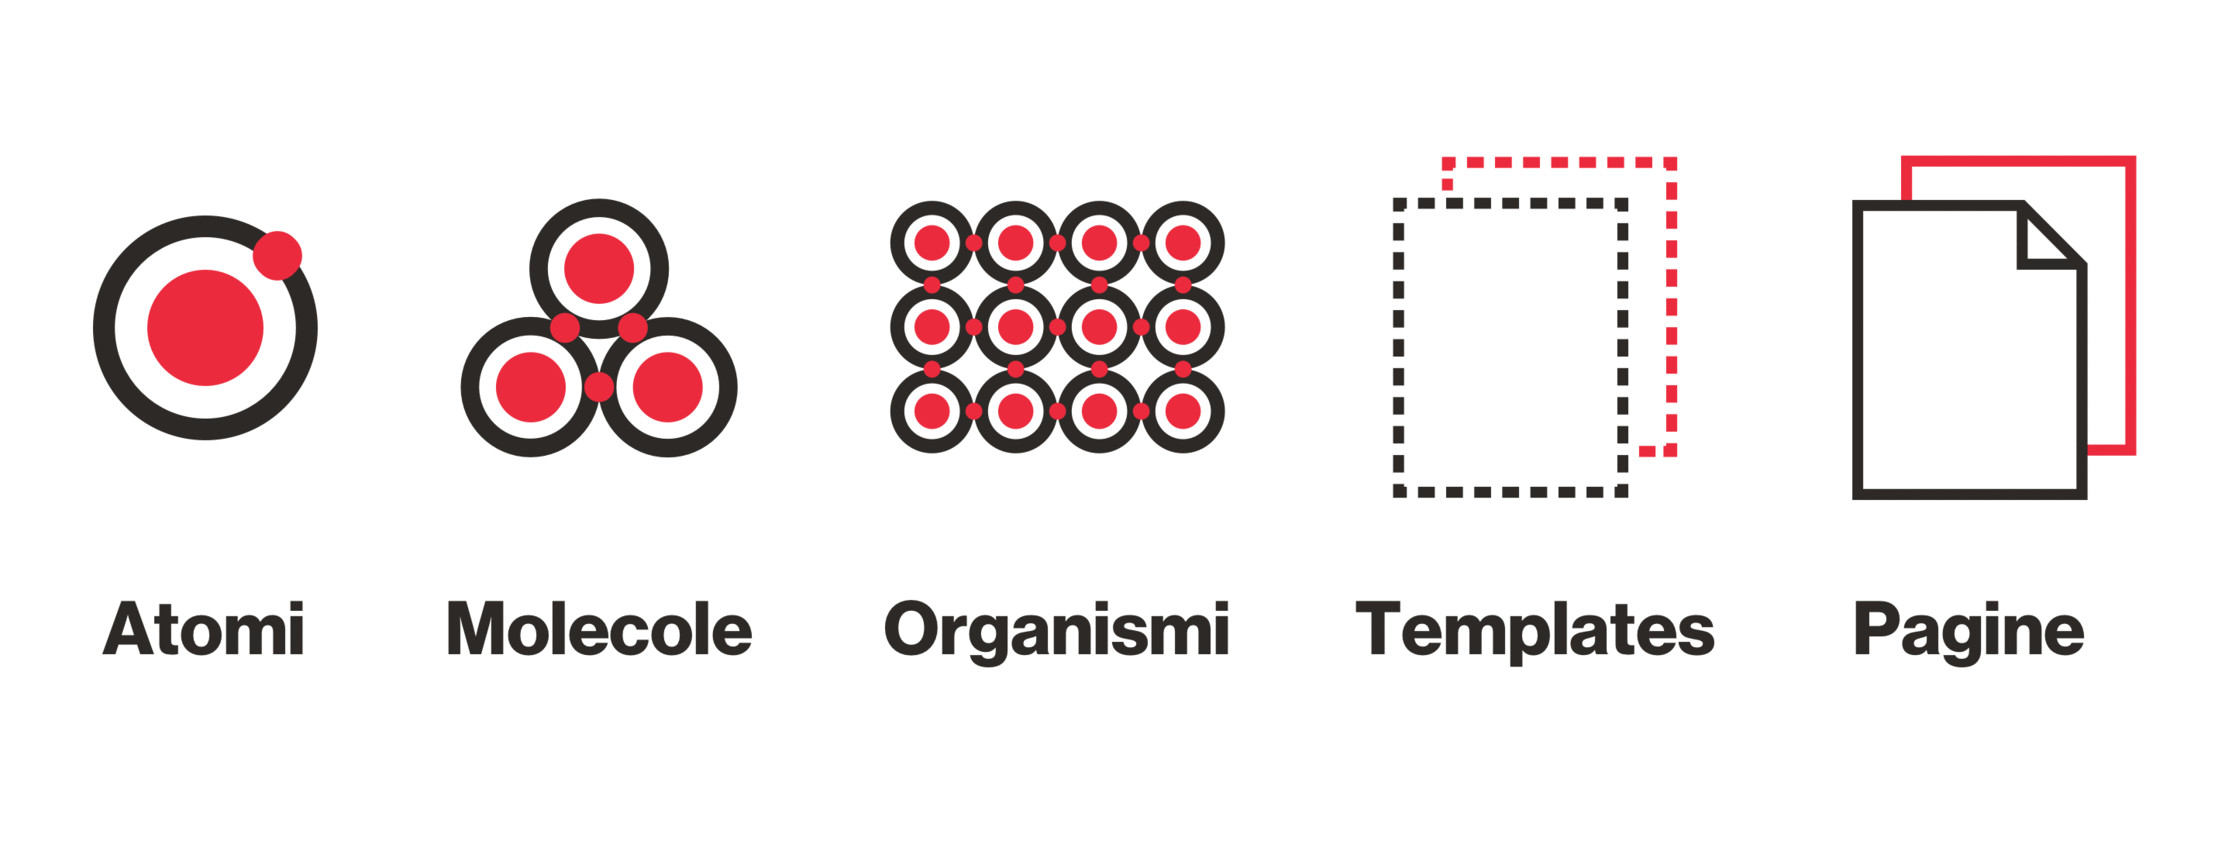
\includegraphics[width=0.8\columnwidth]{atomic} 
	\caption{Elementi atomic design}
\end{figure}
\\

\textbf{Atomi:} in fisica un atomo è la più piccola particella di un elemento che non subisce alterazioni nelle trasformazioni chimiche; nell’Atomic Design gli atomi sono i blocchi fondamentali che comprendono tutta l’interfaccia.
Questi atomi comprendono elementi HTML come tipografia, palette colori, input, bottoni e altri elementi che non possono essere suddivisi ulteriormente senza cessare di essere funzionali.
\\

\textbf{Molecole:} sono semplici gruppi di elementi d'interfaccia che funzionano uniti. Quando combiniamo due oppure più atomi, creiamo quindi una molecola.
\\

Nel contesto della applicazione gli atomi e le molecole sono rappresentate dai elementi della libreria Angular Material, che successivamente sono utilizzate per realizzare l'interfaccia di intera applicazione.

\begin{figure}[!h] 
	\centering 
	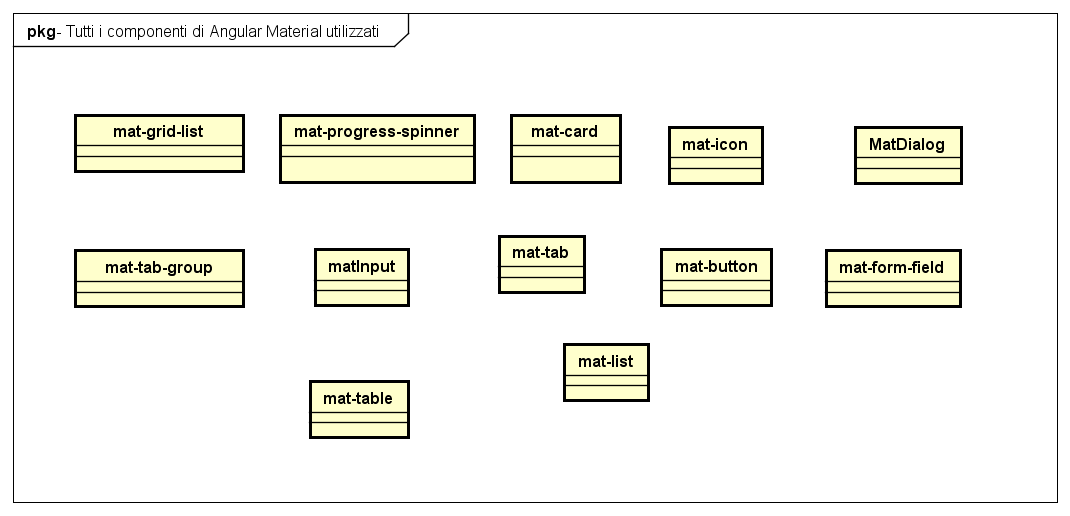
\includegraphics[width=1\columnwidth]{prog/angular} 
	\caption{Componenti Angular Material che formano gli atomi e le molecole dell'applicazione}
\end{figure} 

\textbf{Gli organismi} sono dei componenti più o meno complessi, composti da gruppi di molecole e/o atomi e/o altri organismi. Questi organismi creano diverse sezioni all'interno della nostra interfaccia. Un esempio può essere un menu di navigazione, che è formato in media da diversi pulsanti/link. 
\\

\textbf{I templates} sono creati dall'insieme dai nostri atomi, molecole e organismi. Creando così la prima idea di scheletro della pagina.
\\

\textbf{Le pagine} sono dei templates riempiti di contenuto reale, come immagini, testi, elementi grafici, advertising, ecc. Questo ci aiuta a capire come la pagina, a seconda del caso specifico, si comporterà quando il contenuto andrà a popolarla. 
\subsubsection{Namespace 1} %**************************
Descrizione namespace 1.

\begin{namespacedesc}
    \classdesc{Classe 1}{Descrizione classe 1}
    \classdesc{Classe 2}{Descrizione classe 2}
\end{namespacedesc}


%**************************************************************
\section{Design Pattern utilizzati}

%**************************************************************
\section{Codifica}
             % Product Prototype
% !TEX encoding = UTF-8
% !TEX TS-program = pdflatex
% !TEX root = ../tesi.tex

%**************************************************************
\chapter{Prodotto realizzato}
\label{cap:progetto-terminato}
In questo capitolo verrà spiegata in dettaglio come avviene l’interazione dell'utente Zendesk con l'applicazione
Zendesk e dell'utente Nextep con la pagina degli amministratori.

\section{Editor}
Una volta installata l'applicazione sulla piattaforma Zendesk viene visualizzata automaticamente l'icona dell'applicazione nella sidebar della piattaforma. 
\begin{figure}[!h] 
	\centering 
	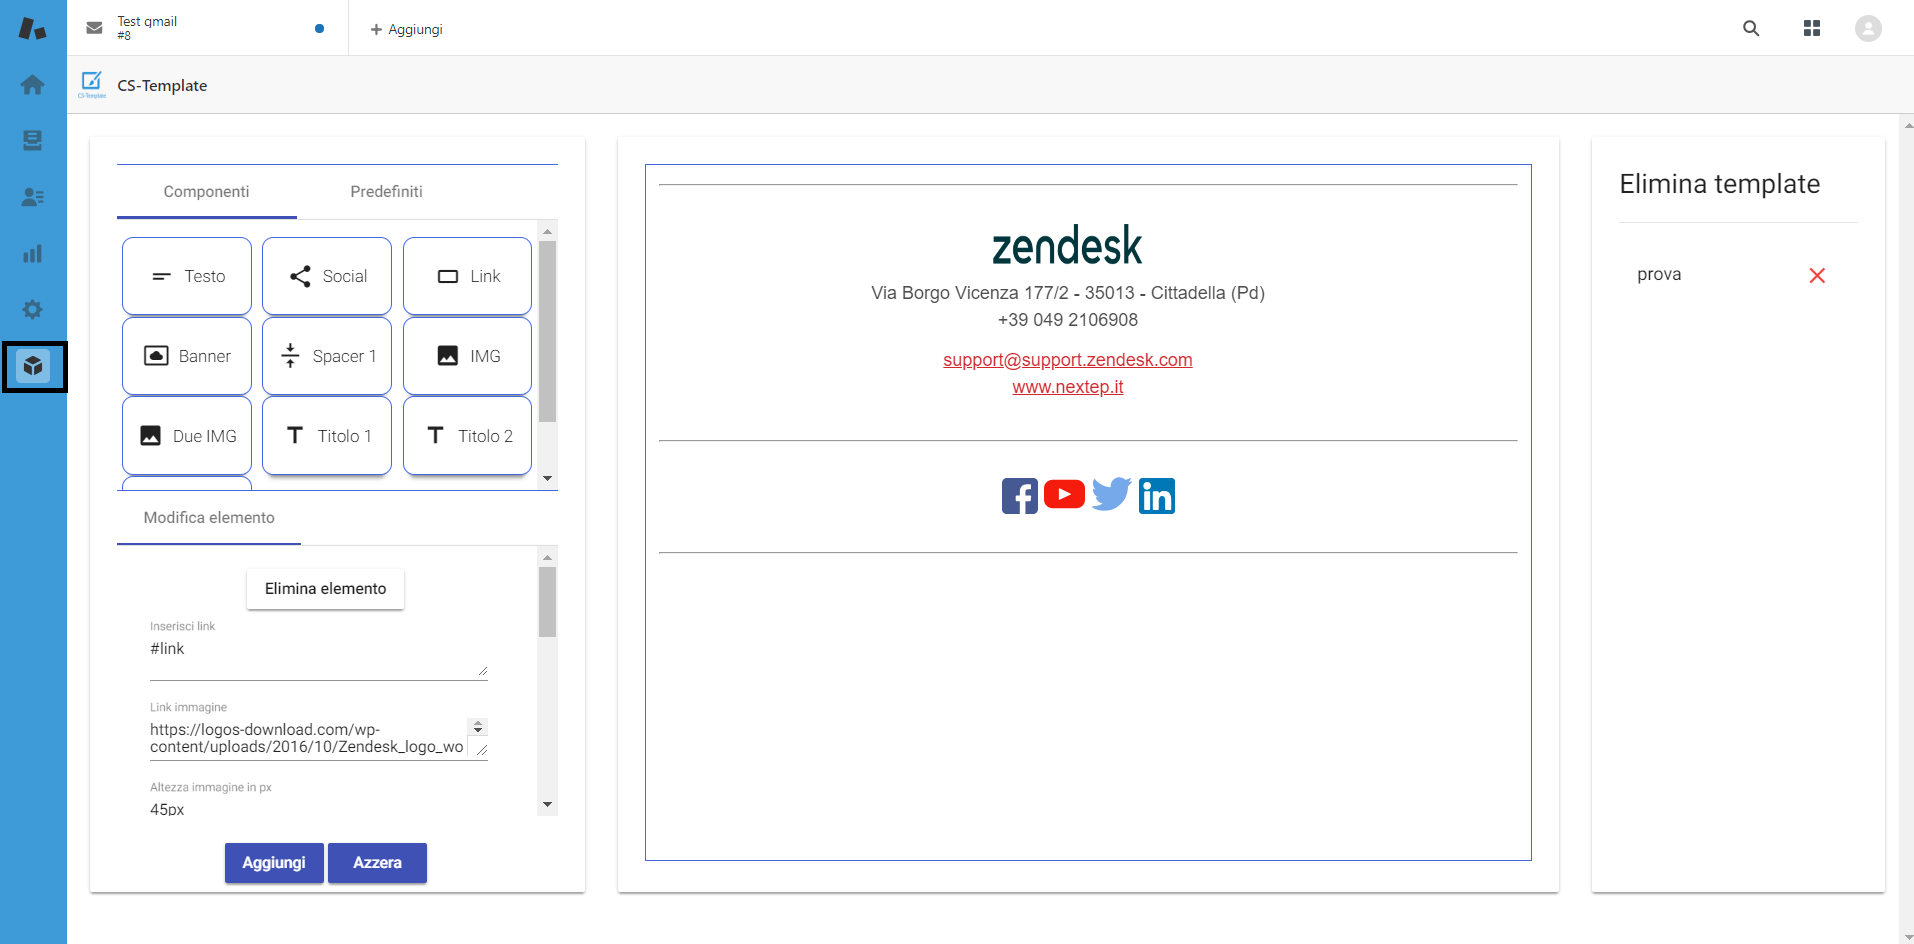
\includegraphics[width=1.2\columnwidth]{editor} 
	\caption{Editor realizzato }
\end{figure}
\begin{itemize}
	\item L'utente può trascinare qualsiasi elemento presente nei "componenti" nel container centrale;
	\item Il container visualizza a schermo il contenuto  HTML e CSS di ogni elemento trascinato in esso;
	\item Facendo doppio click su qualsiasi elemento presente nel container centrale è possibile modificare il suo contenuto oppure eliminarlo dal container;
	\item Gli elementi nel container possono essere ordinati in qualsiasi modo semplicemente facendo drag-and-drop;
	\item E' possibile azzerare il contenuto del container semplicemente cliccando il pulsante "Azzera";
	\item Una volta realizzato il template desiderato l'utente può salvarlo cliccando il pulsante "Aggiungi". Verrà chiesto all'utente di inserire il nome del template, inserendo il nome valido il template verrà automaticamente salvato sul database nosql di Amazon;
	\item A destra nell' "Elimina template" è possibile visualizzare tutti template realizzati e se necessario eliminarli semplicemente cliccano sull'icona "X".  
\end{itemize}
\section{Widget} 
Il widget permette all'agente di Zendesk di utilizzare i template realizzati nelle risposte verso clienti. 
  \begin{figure}[!h] 
  	\centering 
  	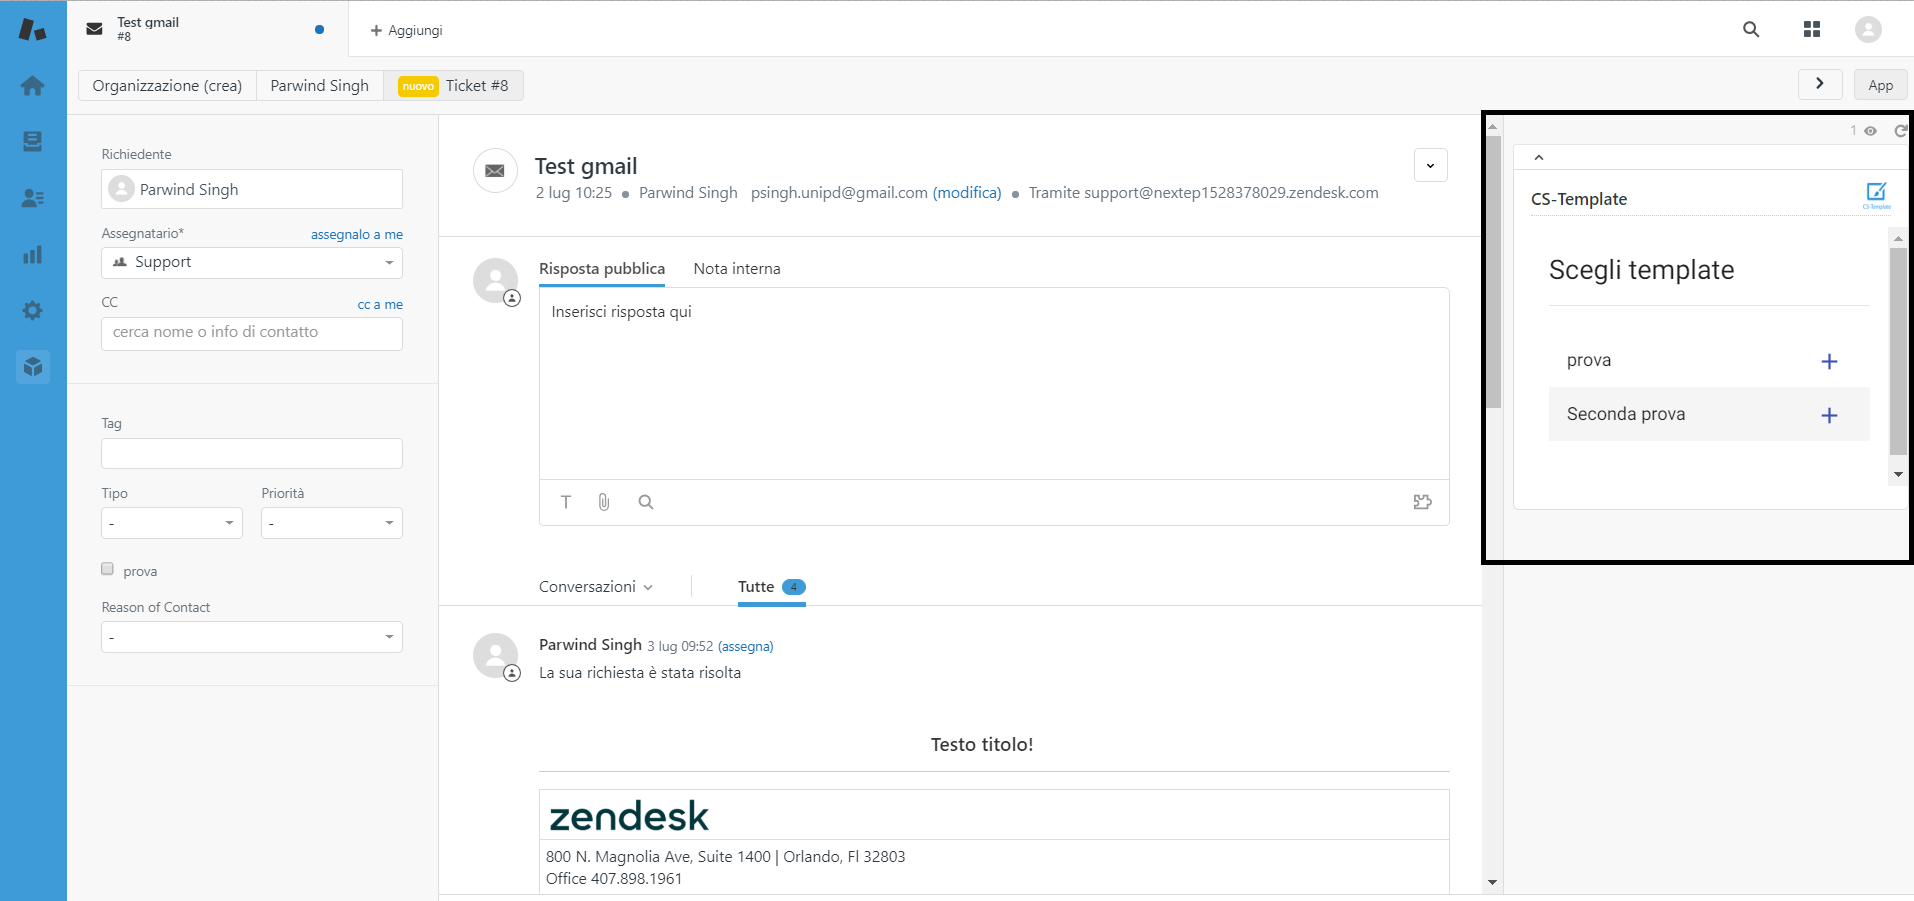
\includegraphics[width=1.2\columnwidth]{widget} 
  	\caption{Editor realizzato }
  \end{figure}
  \begin{itemize}
  	\item L'utente visualizza nel widget tutti i template realizzati;
  	\item L'utente può selezionare il template da utilizzare nella risposta;
  	\item Il template viene automaticamente aggiunto alla risposta. 
  \end{itemize}
\newpage
\section{Pagina di login}
Nella immagine di seguito viene visualizzata il form di login contenuto nella pagina di login. Una volta inseriti i dati corretti, viene automaticamente caricata la pagina degli amministratori. Se i dati inseriti non sono corretti, viene mostrato a schermo un messaggio di errore.
\begin{figure}[!h] 
	\centering 
	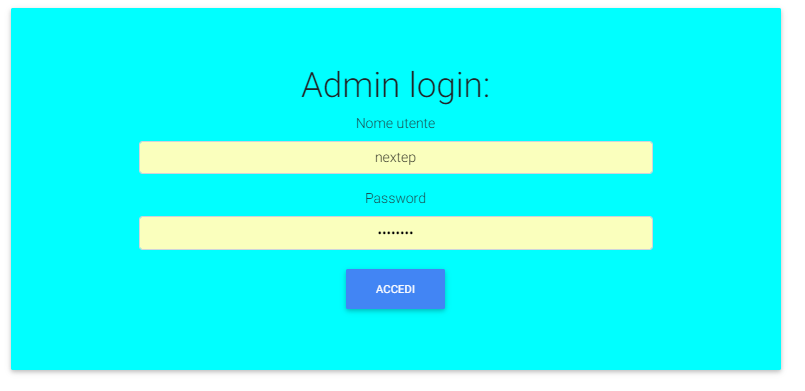
\includegraphics[width=0.8\columnwidth]{login} 
	\caption{Editor realizzato }
\end{figure}
\section{Pagina degli amministratori}
Nella immagine di seguito viene visualizzata la pagina degli amministratori. In questa pagina è possibile aggiungere e rimuovere un cliente di Nextep che utilizza oppure andrà ad utilizzare l'applicazione CS-Template.
\begin{figure}[!h] 
	\centering 
	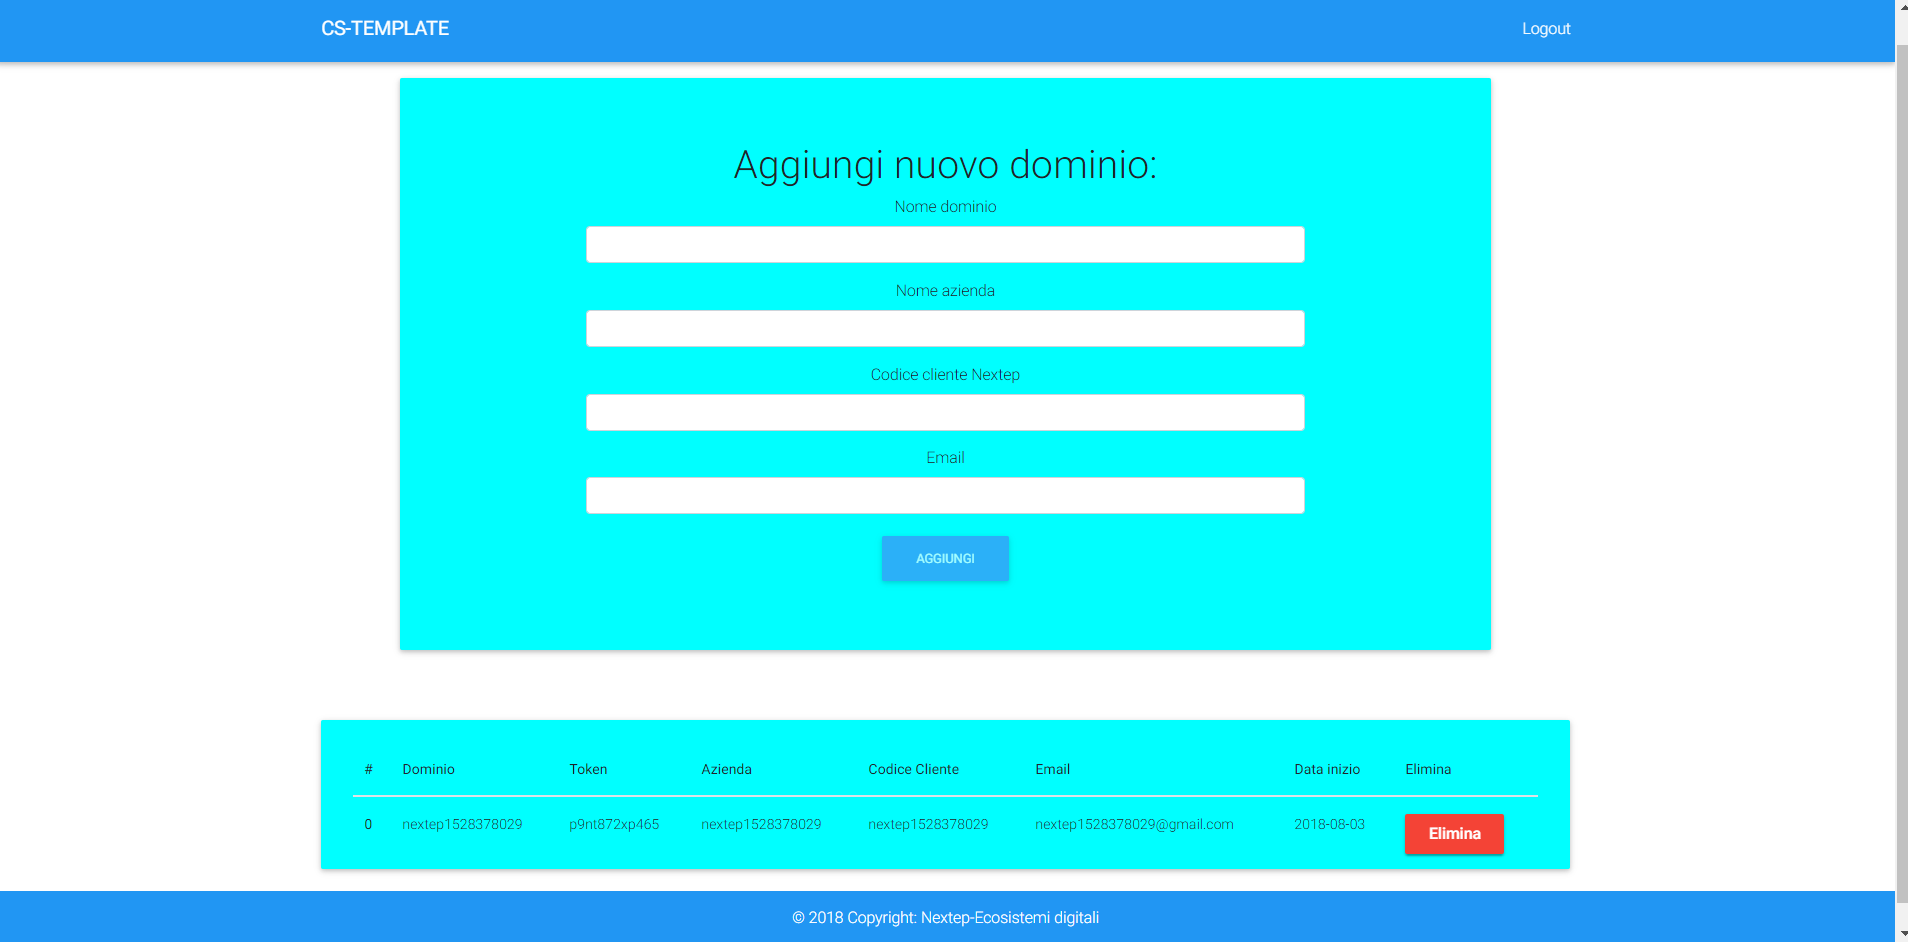
\includegraphics[width=1.2\columnwidth]{admin} 
	\caption{Editor realizzato }
\end{figure}

             % Product Design Freeze e SOP
% !TEX encoding = UTF-8
% !TEX TS-program = pdflatex
% !TEX root = ../tesi.tex

%**************************************************************
\chapter{Valutazione retrospettiva
}
\label{cap:conclusioni}
%**************************************************************
In quest'ultimo capitolo faccio un bilancio dello stage, iniziando da un confronto tra
gli obiettivi prefissati e quelli soddisfatti.
Illustro cosa ho appreso, sia a livello professionale che formativo.
Concludo con una valutazione personale sia sull’esperienza di stage.
%**************************************************************
\section{Raggiungimento degli obiettivi}
Gli obiettivi descritti all'inizio del periodo di stage hanno avuto il seguente risultato:
\begin{center}
	\begin{table}[h]
		\centering
		\begin{tabular}{|c|c|c|ll}
			\cline{1-3}
			\textbf{Tipologia}          & \textbf{Obiettivo} & \textbf{Esito} &  &  \\ \cline{1-3}
			Obbligatorio       & Studio di tutte le tecnologie e la loro integrazione                   & Soddisfatto                   &  &  \\
			\cline{1-3}
			Obbligatorio&  Realizzazione dell'applicazione per la piatttaforma Zendesk                   & Soddisfatto                    &  &  \\
			\cline{1-3}
		Obbligatorio & Realizzazione della pagina degli amministratori                    & Soddisfatto                     &  &  \\ \cline{1-3}
			Obbligatorio   & Utilizzo dei sistemi Cloud per quanto riguarda il lato backend                   & Soddisfatto                    &  &  \\ \cline{1-3}
			Obbligatorio   & Documentazione tecnica di quanto realizzato                   & Soddisfatto                    &  &  \\ \cline{1-3}
		\end{tabular}
	\caption{Raggiungimento obiettvi}
	\end{table}
	\label{tab:Soddisfacimento Requisiti}

\end{center}
	Durante lo stage ho acquisito diverse conoscenze che mi hanno formato
e portato al raggiungimento degli obiettivi prefissati. Di seguito verranno
elencate le conoscenze principali che hanno caratterizzato il periodo svolto
in azienda.
\begin{itemize}
	\item \textbf{Angular:} ho avuto modo di studiare molto bene il framework Angular. Le SPA sono sempre più richieste nella realtà aziendale. 
	\item \textbf{REST API:} ho avuto modo capire molto bene come funzionano le REST API. 
	\item \textbf{AWS:} sicuramente la tecnologia più interessante sono stati i servizi web di Amazon. Sempre più aziende puntano a queste tecnologie. Si sente sempre più parlare dell'architettura serverless utilizzando in frontend Angular, React ecc.
	\item \textbf{Lavoro aziendale:}  ho imparato cosa significa lavorare in un’azienda,
	la suddivisione dei ruoli e l’importanza del lavoro in team. Nel
	contempo ho sviluppato anche la capacità di essere autonomo in certe
	circostanze, in modo da non dipendere costantemente da altre persone.
\end{itemize}
\section{Valutazione personale sullo stage}
In conclusione l’esperienza che ho vissuto durante il periodo di stage è stata
molto formativa ed interessante, soprattutto perché ho potuto affrontare
nuove tematiche rispetto al mio corso di studi in Università. Nonostante
ciò, grazie alle conoscenze apprese durante gli anni di studio, sono riuscito ad
apprendere velocemente quanto necessario per svolgere il progetto. Inoltre,
ho messo alla prova le mie capacità confrontandomi, per la prima volta, con
il mondo del lavoro e posso affermare di essere rimasto molto soddisfatto. Mi è stato fornito tutto il materiale ed
aiuto necessari per svolgere al meglio il mio lavoro ed ho potuto stabilire un
buon rapporto, lavorativo ed umano, con gli altri dipendenti dell’azienda. Al
termine dello stage ho acquisito consapevolezza delle mie capacità e ritengo
che sia stato un ottimo periodo formativo.
             % Conclusioni
\appendix                               
% !TEX encoding = UTF-8
% !TEX TS-program = pdflatex
% !TEX root = ../tesi.tex

%**************************************************************
\chapter{Appendice A}
\section{Servizi di Angular 6}
 Un servizio in Angular 6 è una classe di tipo Singleton che implementa funzionalità condivise dai vari elementi di un’applicazione, siano essi componenti che altri servizi.
Ne esiste solo un istanza di uno servizio per tutta l'applicazione, in questo modo i dati condivisi dai diversi componenti sono gli stessi.
\\

L'implementazione di un servizio aviene utilizando il decorator @Injectable() di Angular. Questo decorator aggiunge alla classe dei metadati che permettono ad Angular di iniettare il servizio nei compoenti come una dipendenza. Viene utilizzato Dependency injection(DI) design pattern per iniettare le dipendenze dei servizi nei componenti. 
\begin{figure}[!h] 
	\centering 
	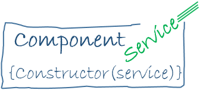
\includegraphics[width=0.5\columnwidth]{DI} 
	\caption{Injector di Angular}
\end{figure}
\\

Dependency injection è utilizzato ovunque nel Framework Angular. In un'applicazione Angular un componente in media consuma molti servizi utilizzando DI, che li fornisce accesso a tutti i metodi e ai dati forniti dal servizio. 
\\ 

Quando un componente viene creato come prima cosa vengono controllate le sue dipendenze. Se il componente dipende da qualche servizio viene generato l'istanza Singleton di tale servizio(se non esiste già), in questo modo vengono soddisfatte tutte le dipendenze del componente prima della sua creazione. 
La Dependency injection è gestito dal oggetto injector di Angular, che ha il semplice compito di soddisfare le dipendenze. 
\begin{figure}[!ht] 
	\centering 
	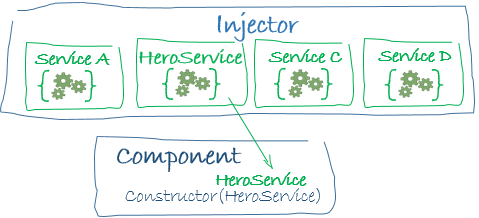
\includegraphics[width=0.7\columnwidth]{DI2} 
	\caption{DI in Angular}
\end{figure}
\section{RxJS in Angular 6}
RxJS (Reactive Extensions for JavaScript) è una libreria di reactive programming che permette di gestire le chiamate asincrone in maniera molto semplice.
\begin{figure}[!ht] 
	\centering 
	
\includegraphics[width=0.5\columnwidth]{rxjs} 
	\caption{Logo di Angular ed RxJS}
\end{figure}             % Appendice A

%**************************************************************
% Materiale finale
%**************************************************************
\backmatter
\printglossaries
% !TEX encoding = UTF-8
% !TEX TS-program = pdflatex
% !TEX root = ../tesi.tex

%**************************************************************
% Bibliografia
%**************************************************************

\cleardoublepage
\chapter{Bibliografia}

\nocite{*}
% Stampa i riferimenti bibliografici
\printbibliography[heading=subbibliography,title={Riferimenti bibliografici},type=book]

% Stampa i siti web consultati
\printbibliography[heading=subbibliography,title={Siti web consultati},type=online]


\end{document}
